%%%%%%%%%%%%%%%%%%%%%%%%%%%%%%%%%%%%%%%%%%%%%%%%%%%%%%%%%%%%%%%%%%%%%%%%%%%%%%%%
% event_selection.tex: Select of showering and tracking events:
%%%%%%%%%%%%%%%%%%%%%%%%%%%%%%%%%%%%%%%%%%%%%%%%%%%%%%%%%%%%%%%%%%%%%%%%%%%%%%%%
\chapter{Problem 2}
\label{Problem 2}
%%%%%%%%%%%%%%%%%%%%%%%%%%%%%%%%%%%%%%%%%%%%%%%%%%%%%%%%%%%%%%%%%%%%%%%%%%%%%%%%
a. the entire system and the forces acting on the elevator, you, and the child are shown
in Figure \ref{fig:partA}

\begin{figure}[h]
	\centering
	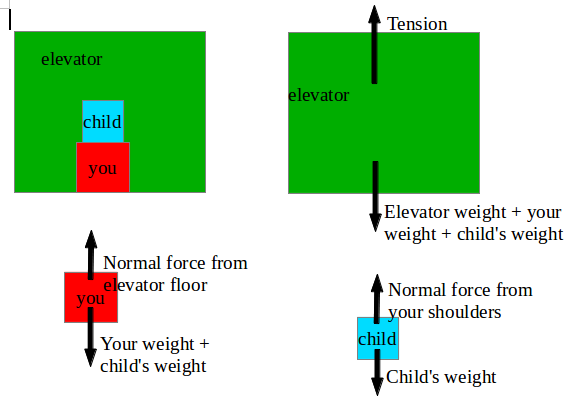
\includegraphics[scale=0.85]{figures/exam2problem2partA_image.png}
	\caption{elevator and two person system, and the forces acting on each person and the elevator.}
	\label{fig:partA}
\end{figure}

b. the tension is $11300$ Newtons
                                              
given the net acceleration $a_{net}$ and the masses of the elevator $m_{elev}$, you $m_{you}$, and
the child $m_{child}$, find the tension T using Newton's law.
$(m_{elev} + m_{you} + m_{child})a_{net}$ = T - $(m_{elev} + m_{you} + m_{child})$g
T = $(m_{elev} + m_{you} + m_{child})(g + a_{net})$ = $(1280.0 kg)(9.81 \frac{m}{s^{2}} - 1.00 \frac{m}{s^{2}})$
T = $11276.8$ Newtons

c. weight force = $196$ Newtons downward   normal force = $176$ Newtons upward
                                                     
weight $m_{child}g = 196$ Newtons
normal force from your shoulders $N_{child} = m_{child}(g + a_{net}) = (20.0 kg)(8.81 \frac{m}{s^{2}})$
$N_{child} = 176$ Newtons

d. weight force = $785$ Newtons downward   normal force = $705$ Newtons upward
                                                           
weight $(m_{you} + m_{child})g = 785$ Newtons
normal force from the floor $N_{you} = (m_{child} + m_{you})(g + a_{net}) = (80.0 kg)(8.81 \frac{m}{s^{2}})$
$N_{you} = 705$ Newtons


%%%%%%%%%%%%%%%%%%%%%%%%%%%%%%%%%%%%%%%%%%%%%%%%%%%%%%%%%%%%%%%%%%%%%%%%%%%%%%%%
